\documentclass[12pt, titlepage]{article}

\usepackage{booktabs}
\usepackage{longtable}
\usepackage{pdflscape}
\usepackage{tabularx}
\usepackage{graphicx}
\usepackage{hyperref}
\usepackage{float}
\usepackage[round]{natbib}

\hypersetup{
    colorlinks,
    citecolor=blue,
    filecolor=black,
    linkcolor=red,
    urlcolor=blue
}

\input{../Comments}
\input{../Common}

\title{User Guide for \progname} 
\author{\authname}
\date{\today}

\begin{document}

\maketitle

\pagenumbering{roman}

\section*{Revision History}

\begin{tabularx}{\textwidth}{p{3cm}p{2cm}X}
\toprule {\bf Date} & {\bf Version} & {\bf Notes}\\
\midrule
04-11-2024 & 1.0 & Initial Version\\
27-03-2025 & 1.1 & Updates based on user feedback\\
\bottomrule
\end{tabularx}

~\newpage

\tableofcontents

\listoffigures

~\newpage

\pagenumbering{arabic}

\section{Introduction}
\subsection{Purpose}
This document serves as the user guide for RapidCare, a healthcare management system designed to streamline patient record management and medical operations. RapidCare addresses the growing shortage of family doctors in Ontario and the resulting strain on emergency rooms by reducing documentation overhead, thus allowing healthcare professionals to focus more on patient care.

\subsection{Scope}
The guide covers installation, setup, and usage of both client and server components of RapidCare. It details the process of patient documentation, voice dictation for medical notes, automated diagnosis and medicine suggestions, and healthcare network management.

\subsection{Overview}
The system consists of:
\begin{itemize}
\item Web-based client interface (React)
\item Python files backend
\item Firebase database
\end{itemize}

RapidCare is built to tackle documentation overhead, which currently consumes a significant portion of healthcare professionals' time. By using voice dictation and AI-assisted documentation, the system aims to reduce paperwork time, increase patient throughput, and improve overall care quality.

\section{Installation}
%Pranav can complete

\newpage

\section{Usage}
\subsection{Client Interface}
\begin{figure}[H]
\centering
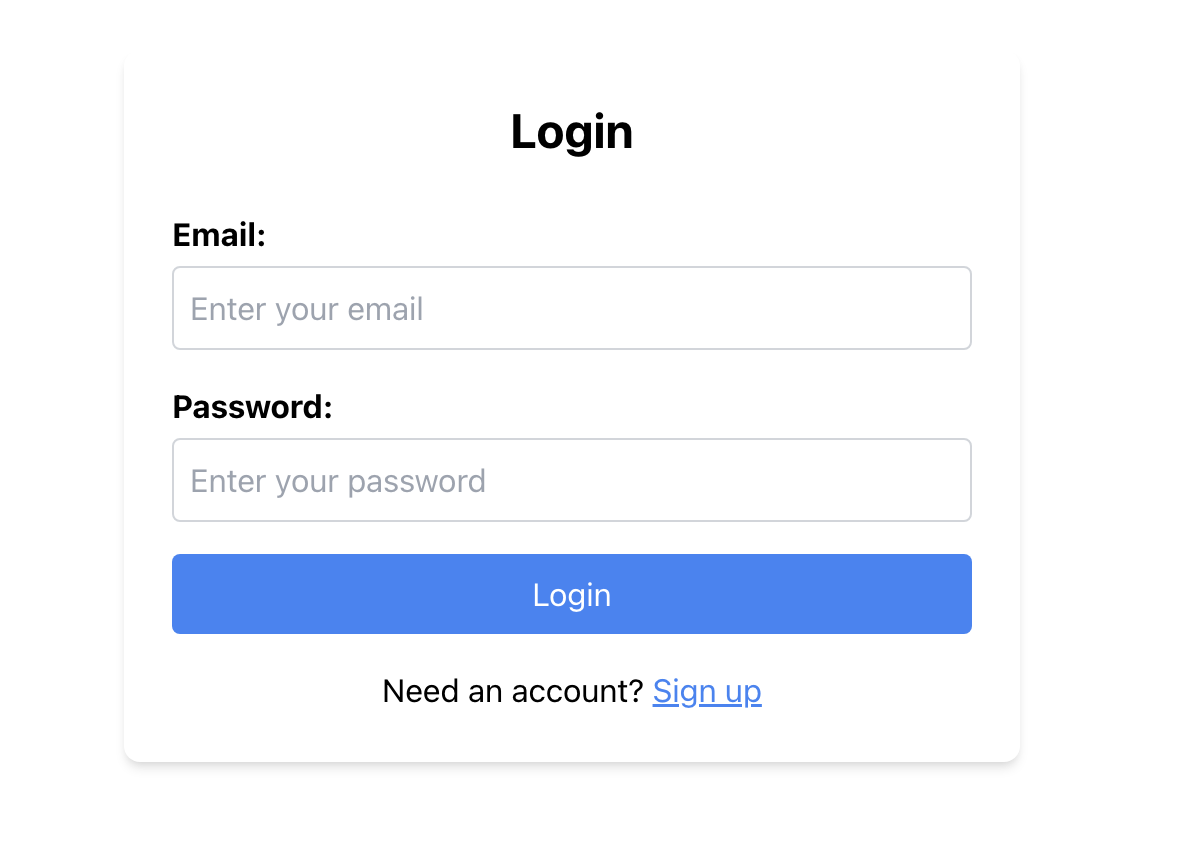
\includegraphics[width=0.8\textwidth]{login.png}
\caption{Login Screen Interface}
\label{fig:login}
\end{figure}

\subsubsection{Logging In}
\begin{itemize}
\item Enter admin/admin-provided credentials
\item Based on credentials users are directed to their respective main page
\item Click "Login" button
\end{itemize}

The system will redirect you to different interfaces based on your selected role:
\begin{itemize}
\item \textbf{Admin}: Directs to the administration dashboard with system-wide management tools
\item \textbf{Healthcare Professionals}: Directs to the hospital main page with their upcoming appointments
\end{itemize}

\subsubsection{Administration Dashboard}
\begin{figure}[H]
\centering
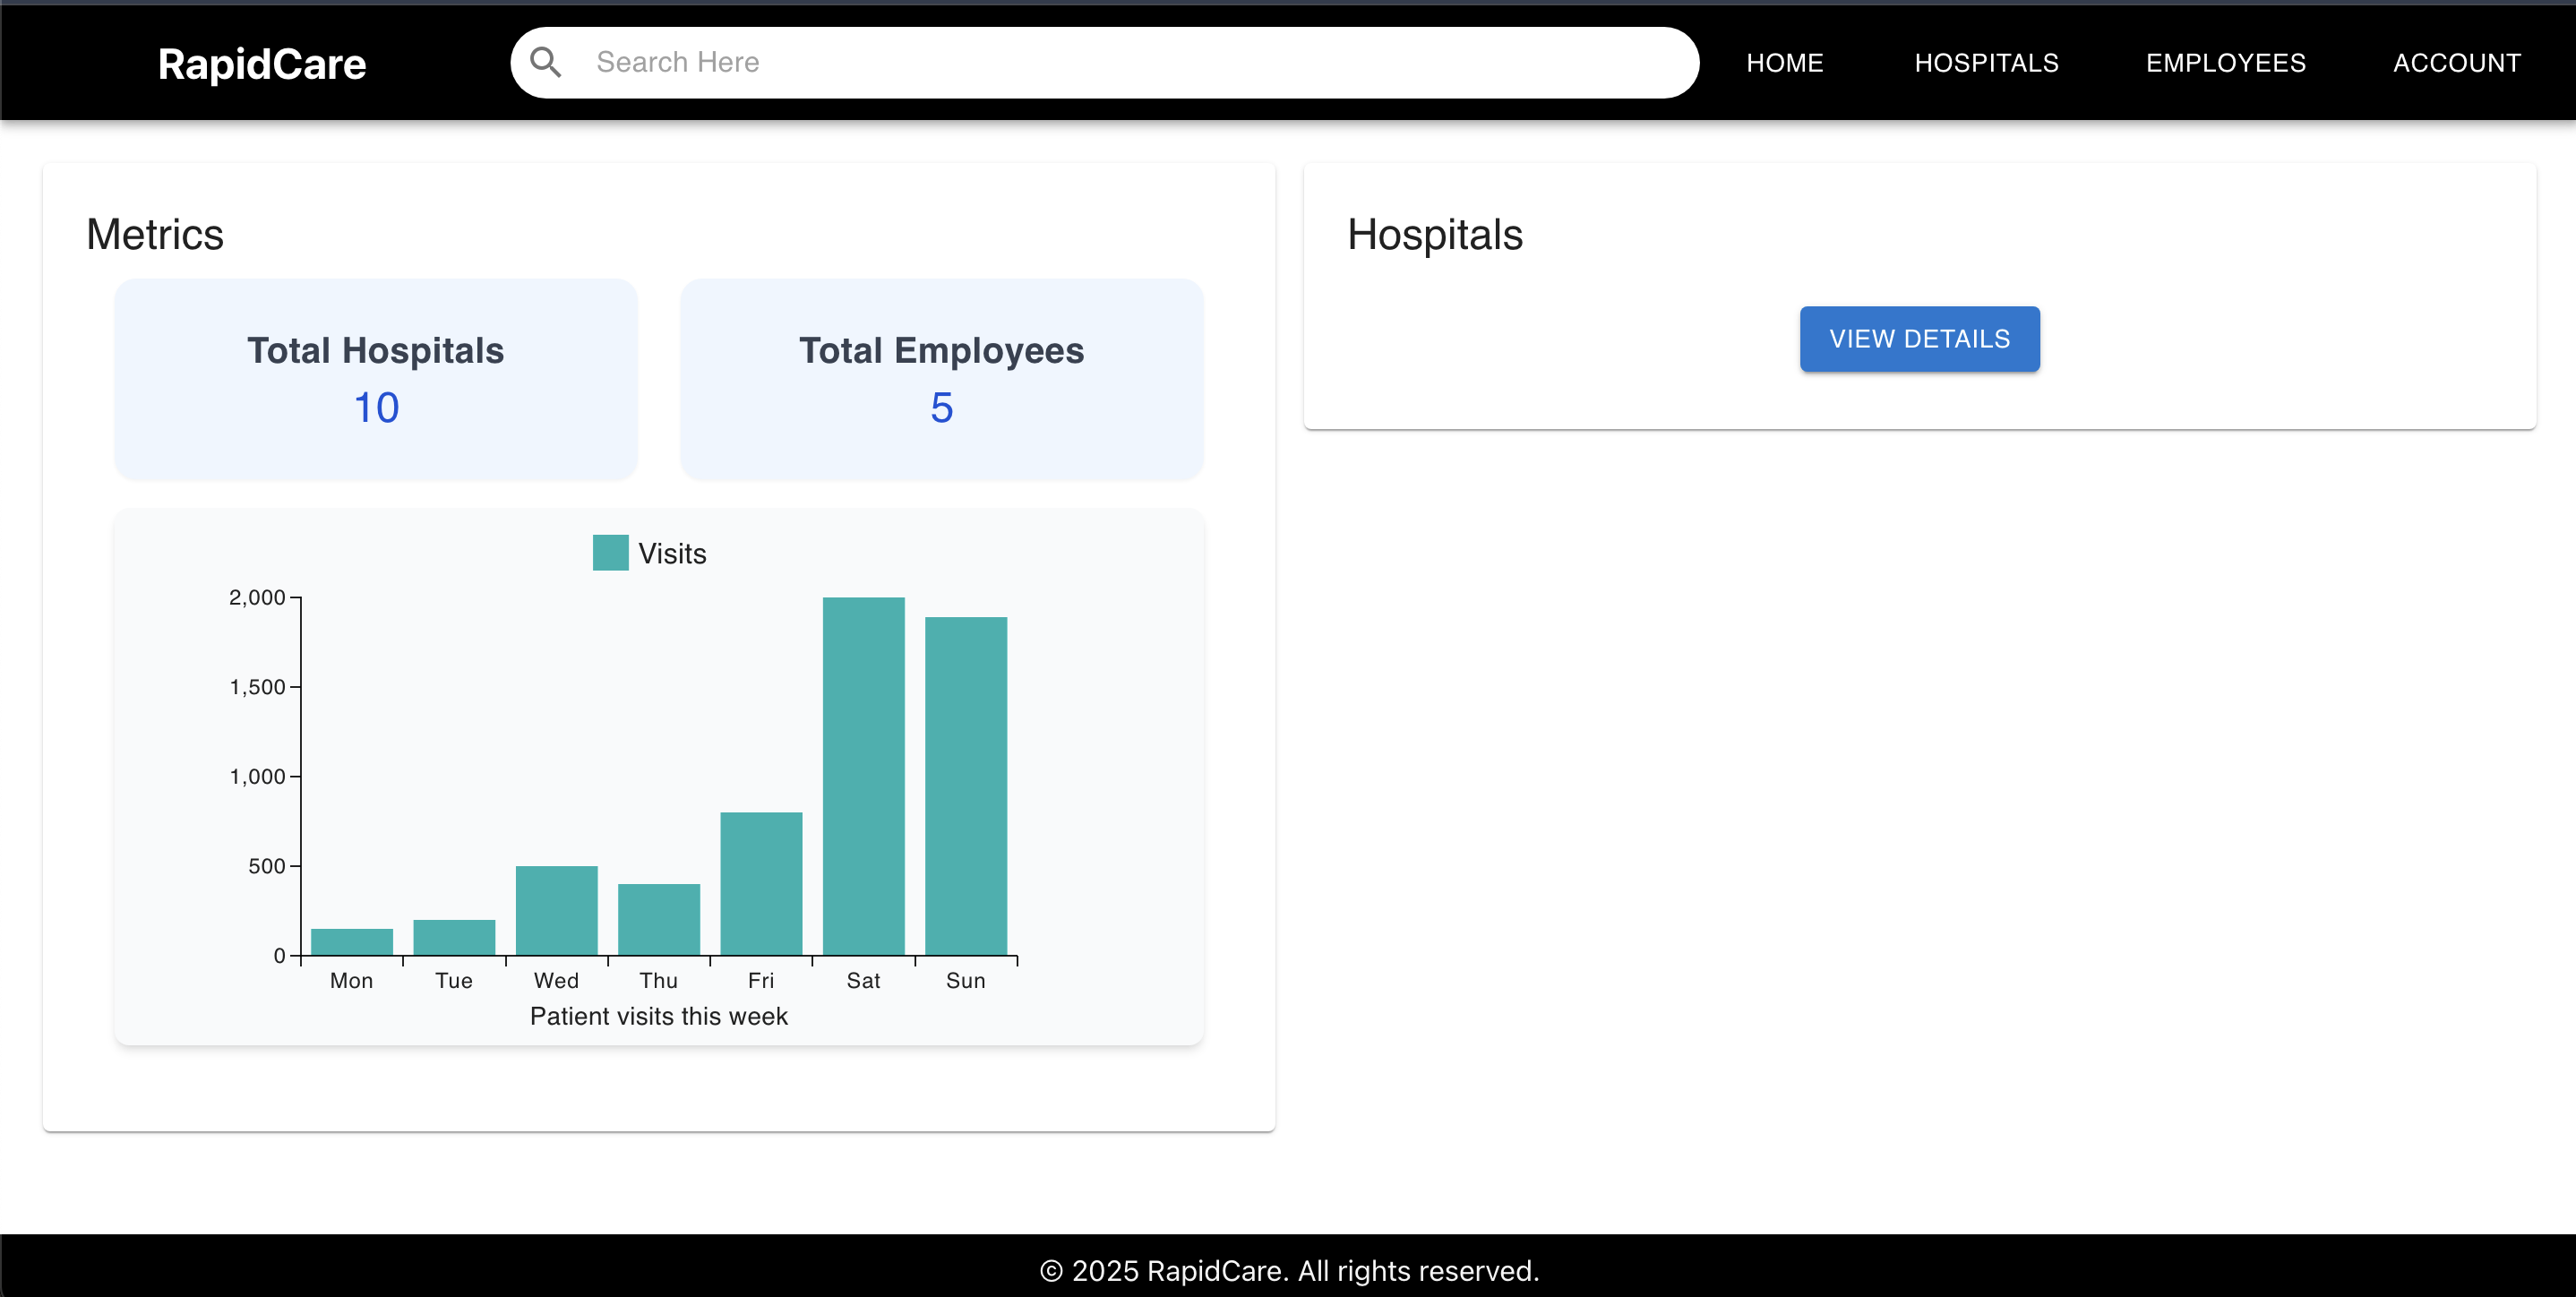
\includegraphics[width=0.8\textwidth]{admin.png}
\caption{Administrator Main Dashboard Interface}
\label{fig:admin_dashboard}
\end{figure}

The Administration Dashboard provides a comprehensive overview of system operations, including:
\begin{itemize}
\item User management controls
\item System performance metrics
\item Hospital network configuration
\item Employee management tools
\item Backup and maintenance utilities
\end{itemize}

The navigation bar provides quick access to:
\begin{itemize}
\item \textbf{Home}: Return to the main dashboard
\item \textbf{Hospitals}: Manage hospital networks
\item \textbf{Employees}: Manage healthcare professionals
\item \textbf{Account}: Edit profile information
\end{itemize}


\subsubsection{Healthcare Professional Dashboard}
\begin{figure}[H]
\centering
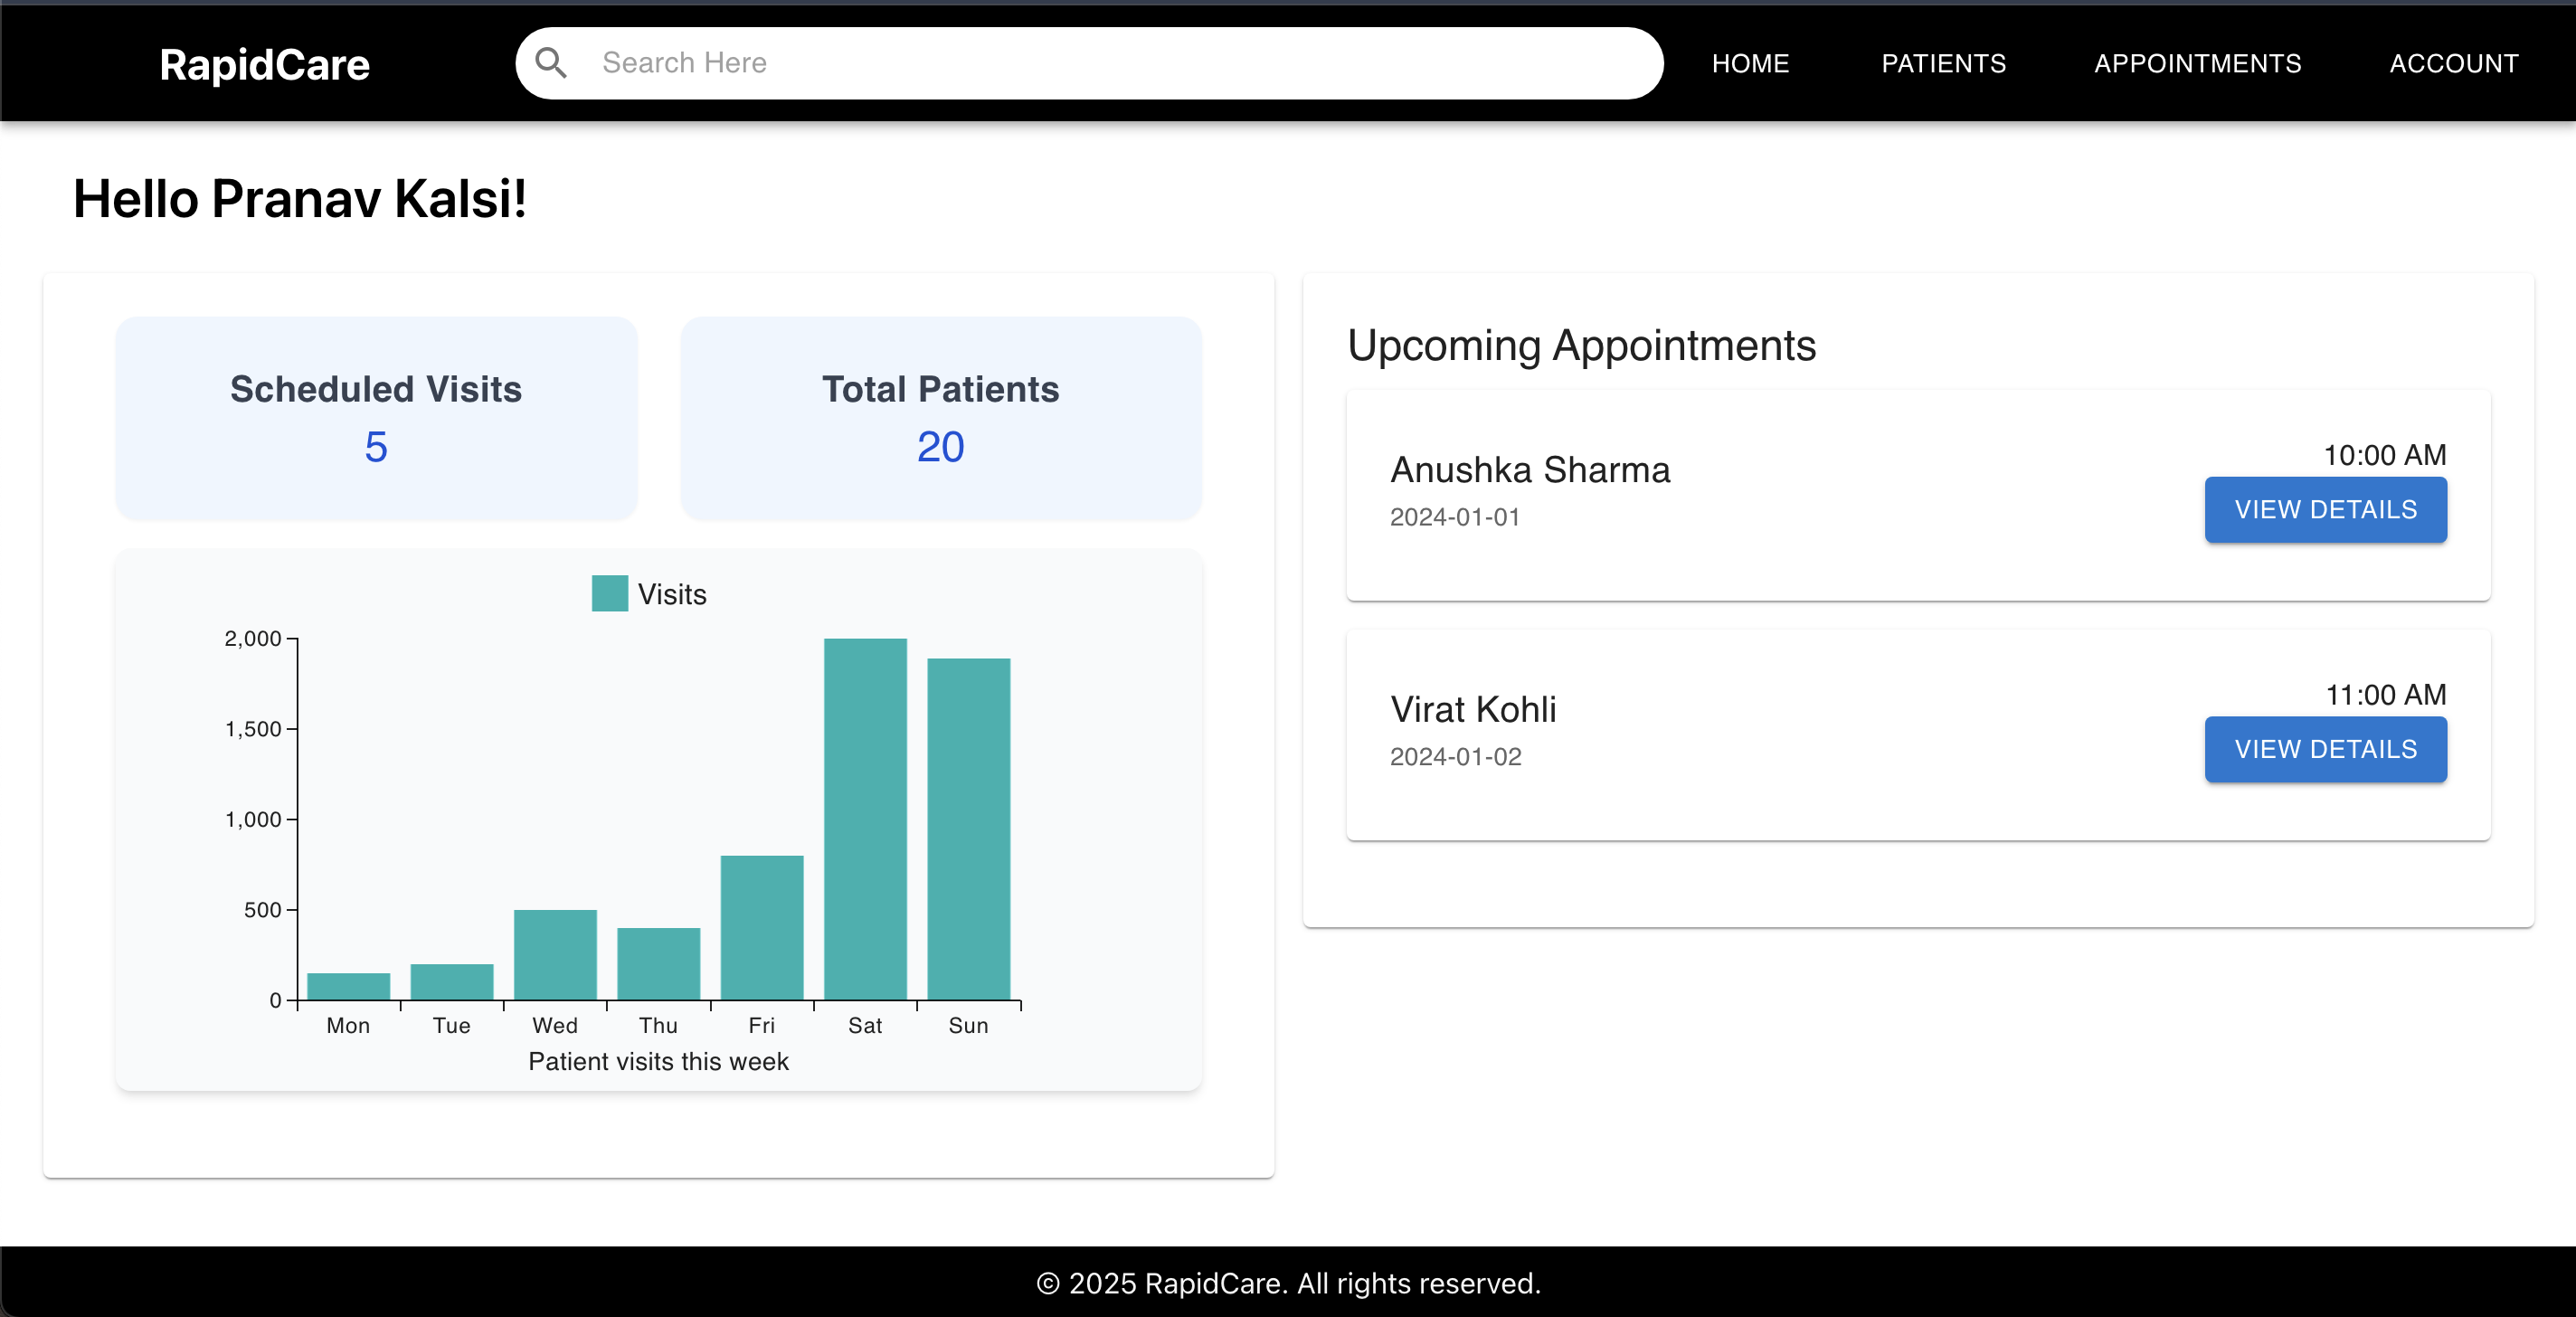
\includegraphics[width=0.8\textwidth]{healthcare.png}
\caption{Healthcare Professional Dashboard Interface}
\label{fig:healthcare_dashboard}
\end{figure}

The Healthcare Professional Dashboard provides an intuitive interface for managing patient care, including:
\begin{itemize}
\item Daily appointment schedule overview
\item Patient visit statistics and trends
\item Quick access to patient records
\item Upcoming appointment notifications
\item Performance metrics and visit analytics
\end{itemize}

The navigation bar provides quick access to:
\begin{itemize}
\item \textbf{Home}: Return to the main dashboard
\item \textbf{Patients}: Access comprehensive patient records
\item \textbf{Appointments}: Manage and schedule patient appointments
\item \textbf{Account}: Edit profile information.
\end{itemize}

\subsubsection{Patient Management}
\begin{longtable}{p{0.3\textwidth}p{0.6\textwidth}}
\toprule
\textbf{Action} & \textbf{Steps} \\
\midrule
Add Patient & Click "+ Add Patient", Complete Form, "Create Patient" \\
View Records & Search for patient, "View Record" \\
Edit Information & Click any field, "Edit", Make Changes, "Save" \\
Remove Patient & Open Patient Records, "Delete Profile", Confirm Deletion \\
\bottomrule
\end{longtable}

\subsection{Voice-to-Text Transcription}
RapidCare's voice dictation feature allows you to automatically transcribe patient-provider conversations:

\begin{enumerate}
\item Open the relevant patient record
\item Click "Start Recording" to initiate dictation
\item Speak clearly to record your conversation with the patient
\item When finished, click the "Stop Recording"
\item Review the transcribed text for accuracy
\item Edit any inaccuracies if needed
\item Click "Save" to save the transcription to the patient's chart
\end{enumerate}

\subsection{Text Classification}
After transcribing the patient conversation, RapidCare's text classification model processes the content:
\begin{enumerate}
\item The system automatically analyzes the transcribed text using natural language processing
\item Key symptoms, conditions, and medical terminology are identified and highlighted
\item The system categorizes the content into relevant sections.
\item Important medical entities are extracted and organized in a structured format
\item The processed text is prepared for the diagnosis suggestion engine
\item The structured data is stored alongside the raw transcription for comprehensive record-keeping
\end{enumerate}

\subsection{Diagnosis and Medicine Suggestions}
After transcribing your conversation with a patient:

\begin{enumerate}
\item The system will automatically analyze the transcribed text
\item RapidCare will suggest possible diagnoses based on the symptoms mentioned
\item Review the diagnosis provided
\item A plan is provided including medication and future plan
\item Review the diagnosis suggestions and plan and make any necessary modifications
\item Confirm the diagnosis and treatment plan to add to the patient's chart by clicking "Save"
\end{enumerate}

\subsection{AI Assist Tool}

AI Assist feature empowers healthcare professionals to quickly gather relevant insights:

\begin{enumerate} 
\item View the patient's records to access their information. 
\item Click the AI Assist button to initiate the query. 
\item Ask any question related to the patient’s data,
\item The AI will rapidly analyze the data and provide a concise response. 
\item Review the AI-generated response and incorporate them into the clinical decision-making process. 
\item Click the "X" button to get out of AI Assist
\end{enumerate}

\subsection{Managing Hospitals}
For hospital administrators:

\subsubsection{Adding a Hospital}
\begin{enumerate}
\item Log in with administrator credentials
\item Navigate to "Hospitals"
\item Click "Add New Hospital"
\item Complete all required fields
\item Click "Save" to add the hospital
\end{enumerate}

\subsubsection{Updating Hospital Information}
\begin{enumerate}
\item Navigate to "Hospitals"
\item Select the hospital to update
\item Click "Edit" button
\item Edit the necessary fields
\item Click "Save" to save changes
\end{enumerate}

\subsubsection{Removing a Hospital}
\begin{enumerate}
\item Navigate to "Hospitals"
\item Select the hospital to remove
\item Click "Delete" button
\item Confirm the deletion when prompted
\end{enumerate}

\subsection{Managing Healthcare Professionals}
For hospital administrators:

\subsubsection{Adding Healthcare Professionals}
\begin{enumerate}
\item Navigate to "Employees"
\item Click "Add Healthcare Professional"
\item Complete all required fields
\item Set up initial credentials
\item Click "Save" to add the professional
\end{enumerate}

\subsubsection{Updating Employee Information}
\begin{enumerate}
\item Navigate to "Employees"
\item Select the employee to modify
\item Click "Edit" button
\item Edit the necessary information
\item Click "Save" to save changes
\end{enumerate}

\subsubsection{Removing an Employee}
\begin{enumerate}
\item Navigate to "Employees"
\item Search for the employee
\item Select the professional to remove
\item Click "Delete" button
\item Confirm the deletion when prompted
\end{enumerate}

\subsection{Server Management}
\subsubsection{Startup Options}
\begin{verbatim}
node server.js --port 3001 --db-config firebaseConfig.json
\end{verbatim}

\subsubsection{Admin Commands}
\begin{tabularx}{\textwidth}{lX}
\toprule
\textbf{Command} & \textbf{Description} \\
\midrule
\texttt{backup create} & Create database backup \\
\texttt{users list} & List all system users \\
\texttt{server restart} & Gracefully restart server \\
\bottomrule
\end{tabularx}

\section{Troubleshooting}
\subsection{Common Issues}
\begin{longtable}{p{0.3\textwidth}p{0.6\textwidth}}
\toprule
\textbf{Symptom} & \textbf{Solution} \\
\midrule
Login failures & Verify credentials, check caps lock \\
Slow performance & Clear browser cache, check network \\
Server crashes & Check logs, verify Firebase connection \\
Transcription errors & Speak clearly, reduce background noise, review and edit transcriptions \\
\bottomrule
\end{longtable}

\subsection{Error Messages}
\begin{itemize}
\item \textbf{ERR\_CONNECTION\_REFUSED}: Server may be down or unreachable
\item \textbf{404 Not Found}: Verify URL or resource path
\item \textbf{503 Service Unavailable}: Check server status
\item \textbf{Authentication Failed}: Verify your credentials
\end{itemize}

\section{Maintenance}
\subsection{Backup Procedures}
\begin{enumerate}
\item Run \texttt{backup create} command
\item Store backup files securely in an off-site location
\item Verify backup integrity regularly by performing test restorations
\item Maintain a backup schedule to ensure data safety
\end{enumerate}

\subsection{Updates}
\begin{itemize}
\item Check GitHub for new releases
\item Follow upgrade instructions
\item Test updates in staging environment first
\item Schedule updates during off-peak hours to minimize disruption
\end{itemize}

\section*{Acknowledgment}
The RapidCare development team thanks all users for their feedback and support in improving the system. Our goal is to reduce documentation overhead for healthcare professionals, enabling them to focus more on patient care and less on paperwork. Your continued feedback helps us enhance the system for better healthcare delivery.

\end{document}